\documentclass[UTF8]{ctexart}
\usepackage{ctex}
\usepackage{geometry}
\geometry{left=3.18cm,right=3.18cm,top=2.54cm,bottom=2.54cm}
\usepackage{graphicx}
\usepackage{framed}
\usepackage{fancyhdr}
\usepackage{setspace}
\pagestyle{fancy}%清除原页眉页脚样式
\fancyhf{}
\fancyhead[C]{华中科技大学电信学院}
\fancyfoot[C]{\thepage}
% \pagestyle{plain}
\begin{document}
\begin{center}
    \quad \\
    \quad \\
    % \kaishu \fontsize{35}{5} \textbf{华 中 科 技 大 学}
    % \vskip 3cm
    \fangsong \fontsize{49}{5}《通信电子线路》实验报告
    \vskip 3cm
    \heiti \zihao{1}\textbf{高频LC}
    \fangsong \zihao{1} 振荡器仿真
\end{center}

\makeatletter
\newcommand\dlmu[2][4cm]{\hskip1pt\underline{\hb@xt@ #1{\hss#2\hss}}\hskip3pt}
\makeatother

\vskip 3cm
\begin{center}
    \zihao{3}
    \begin{tabular}{rl}
         & \makebox[4em][s]{学生姓名}	\hspace{0.2cm}	\dlmu[9cm]{赵展}
         \\
         & \makebox[4em][s]{学号}	\hspace{0.2cm}	\dlmu[9cm]{U202117282}
         \\
         & \makebox[4em][s]{专业班级}	\hspace{0.2cm}		\dlmu[9cm]{种子2101班}
         \\
         & \makebox[4em][s]{实验平台}	\hspace{0.2cm}		\dlmu[9cm]{Multisim 14.3 on Windows}
         \\
    \end{tabular}
    \vskip 3cm
    2023年11月1日
\end{center}

\newpage
\tableofcontents
\newpage

\section{实验目的}
\begin{itemize}
    \item 进一步熟悉NIMultisim电路仿真软件的使用
    \item 掌握高频振荡器的电路结构特点及工作原理
    \item 熟悉高频振荡器的起振过程与震荡波形
\end{itemize}
\section{实验内容}
\begin{itemize}
    \item 使用NIMultisim 绘制两种高频振荡器仿真电路(串/并联改进型电容三端LC 振荡器、串/并联晶体振荡器)
    \item 进行时域仿真,观察时域波形
    \item 进行频域仿真,显示主要关键点的频谱
    \item 要求振荡频率至少为10MHz
\end{itemize}
\section{实验原理}
\subsection{并联改进型电容三端式电路}
并联改进型电容三端式电路的原理图如图\ref{img:1}所示,在电感L的两端并联了一个小电容$C_4$,且满足C1,C2远大于C3,所以其回路等效电容为:
$$
C=\frac{C_1C_2C_3}{C_1C_2+C_2C_3+C_1C_3}+C_4\approx C_3+C_4
$$
反馈系数$F=\frac{C_1}{C_2}$,通常取$\frac{1}{8}$-$\frac{1}{2}$,其震荡频率为:
$$
f_0=\frac{1}{\sqrt{LC}}\approx \frac{1}{2\pi\sqrt{L(C_3+C_4)}}
$$
在实际工作中,电路中$C_3$的选择要合理,$C_3$过小时,振荡管与回路间的耦合过弱,振幅平衡
条件不易满足,电路难于起振,$C_3$过大时,频率稳定度会下降。所以,应该在保证起振条件得
到满足的前提下,尽可能地减小电容$C_3$的值。
\begin{figure}[htbp]
    \centering
    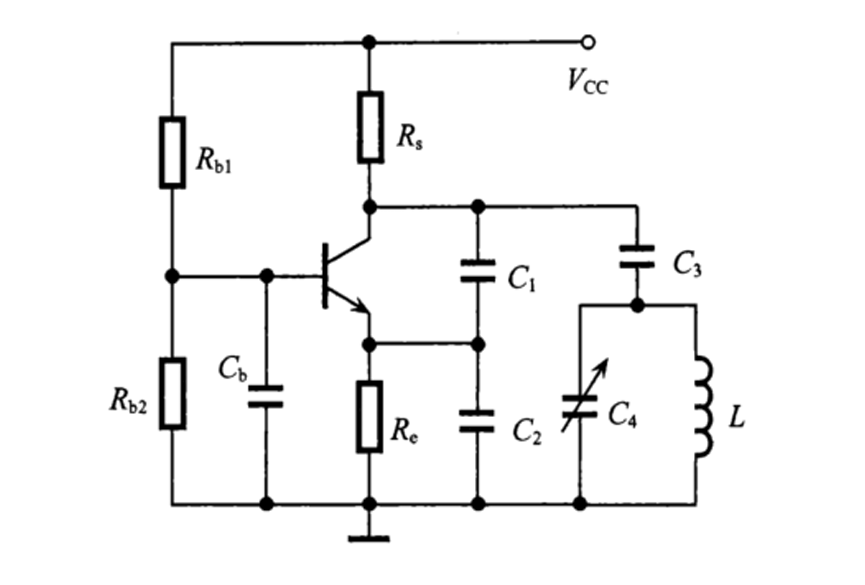
\includegraphics[width=0.8\textwidth]{1.png}
    \caption{并联改进型电容三端式电路原理图}
    \label{img:1}
\end{figure}
根据并联改进型电容三端式电路原理图,在Multisim中搭建实验电路如图\ref{img:2}所示
$C_6$用于过滤输出的直流偏置,$V_2$用于产生白噪声以引
起震荡,为了便于电路实验,将$C_1$和$C_4$设置为可变电容并入电路。
实际工作中,电路中$C_3$的选择要合理,$C_3$过小时,振荡管与回路间的耦合过弱,振幅平衡
条件不易满足,电路难于起振,$C_3$过大时,频率稳定度会下降。所以,应该在保证起振条件得
到满足的前提下,尽可能地减小电容$C_3$的值。
\begin{figure}[htbp]
    \centering
    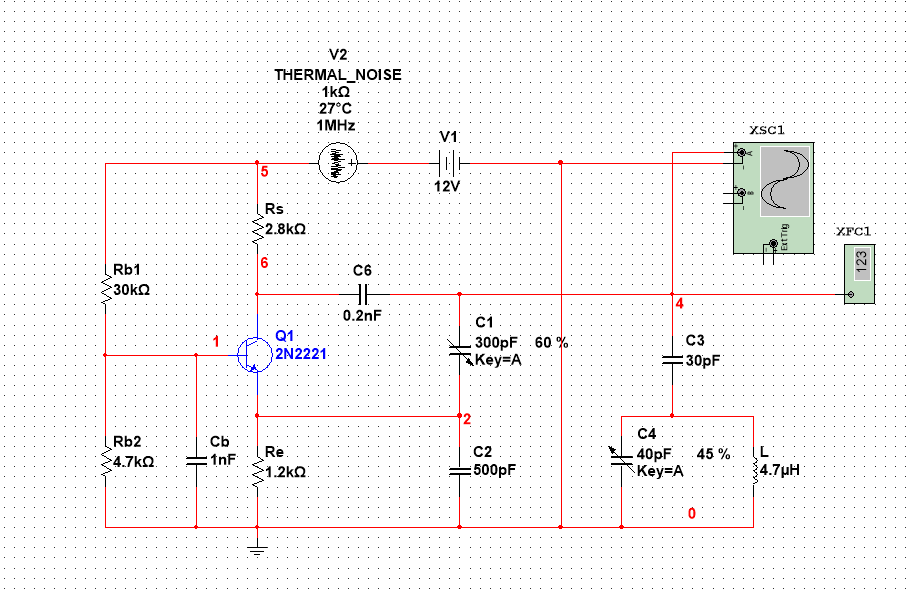
\includegraphics[width=0.8\textwidth]{2.png}
    \caption{并联改进型电容三端式仿真电路}
    \label{img:2}
\end{figure}

\subsection{并联型晶体振荡器}
并联型晶体振荡器电路(又称皮尔斯电路)的原理图如图\ref{img:3}所示:
在石英晶振中,$C_q$极小,$Q_q$极高,所以皮尔斯电路的振荡回路与晶体管和负载之间的耦合非常弱,电路中的不稳定参数对振荡回路的影响很小,提高了回路的标准性;
振荡频率几乎由石英晶振的参数决定,振荡频率
$$
f_0=\frac{1}{a\pi\sqrt{L_q \frac{C_q{C_0+C_L}}{C_q+C_0+C_L}}}=f_q\sqrt{1-\frac{C_q}{C_0+C_L+C_q}}
$$
其中$C_L$是和晶振两端并联的外电路各电容的等效值。
\begin{figure}[htbp]
    \centering
    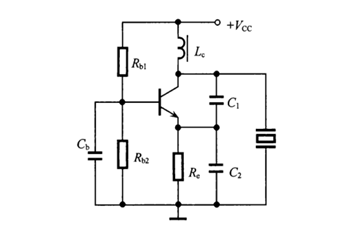
\includegraphics[width=0.8\textwidth]{3.png}
    \caption{并联型晶体振荡器电路原理图}
    \label{img:3}
\end{figure}
根据并联型晶体振荡器电路的原理图,在Multisim中搭建实验电路如图\ref{img:4}所示:
\begin{figure}[htbp]
    \centering
    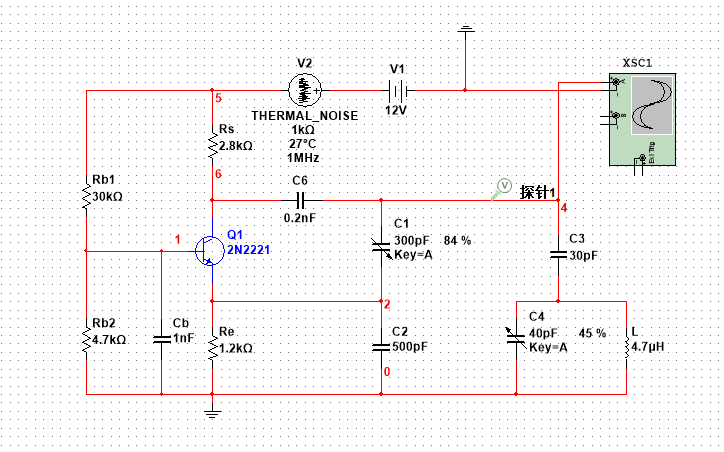
\includegraphics[width=0.8\textwidth]{4.png}
    \caption{并联型晶体振荡器仿真电路}
    \label{img:4}
\end{figure}
\section{实验步骤}
\begin{enumerate}
    \item 按照原理图,搭建仿真电路。
    \item 对于并联改进型电容三端式电路,改变$C_1$的值,进行瞬态分析,观测到起振时间
    \item 对于并联型晶体振荡器电路使用频率计数器,验证振荡频率是否大于10MHz
\end{enumerate}
\section{实验结果与分析}

\subsection{并联改进型电容三端式振荡}
\subsubsection{输出信号电压}
对搭建好的仿真电路进行瞬态分析,得到如图\ref{img:5}所示的结果,在大约8$\mu s$之后电压明显开始增大,在30$\mu s$之后电压逐渐稳定
\begin{figure}[htbp]
    \centering
    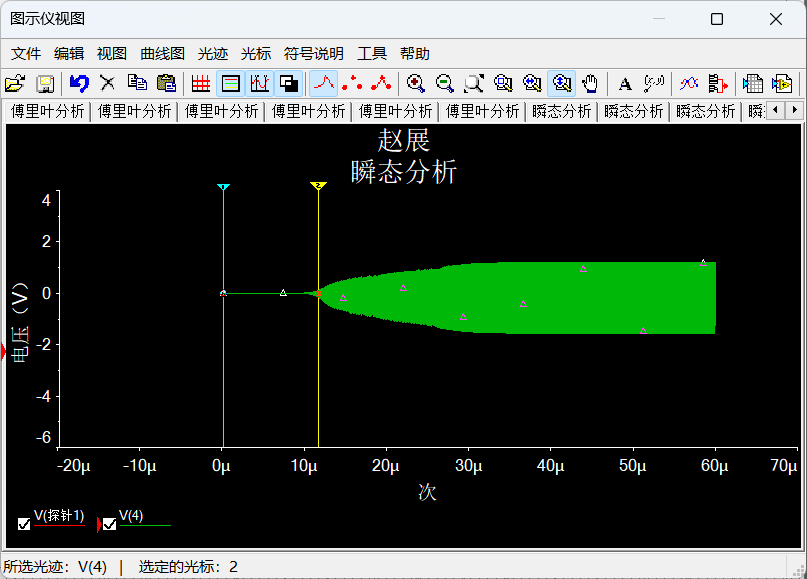
\includegraphics[width=0.8\textwidth]{5.png}
    \caption{瞬态分析:输出电压信号波形}
    \label{img:5}
\end{figure}
对输出信号进行傅里叶分析得到如图\ref{img:16}所示的结果
\begin{figure}[htbp]
    \centering
    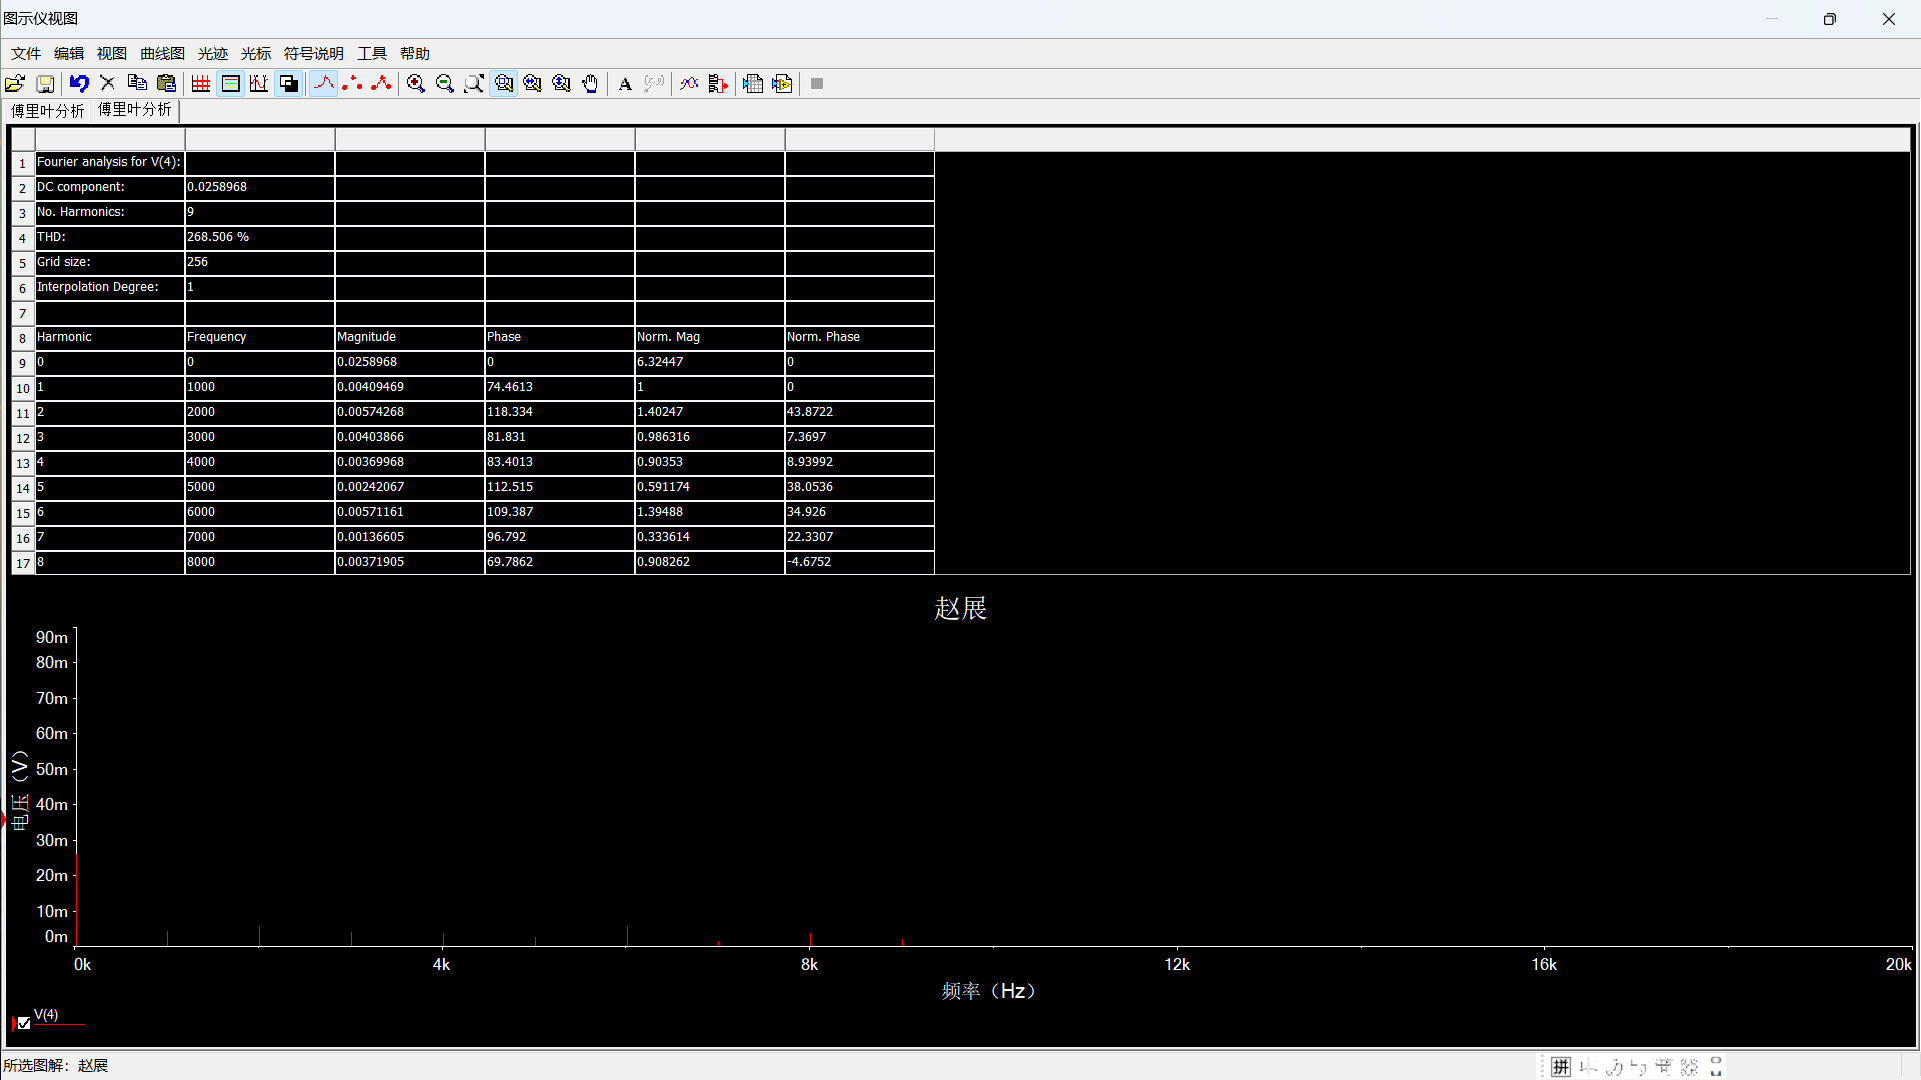
\includegraphics[width=0.8\textwidth]{16.png}
    \caption{傅里叶分析:输出电压信号频谱}
    \label{img:16}
\end{figure}
\subsubsection{反馈系数F对起振的影响}
\begin{figure}[htbp]
    \centering
    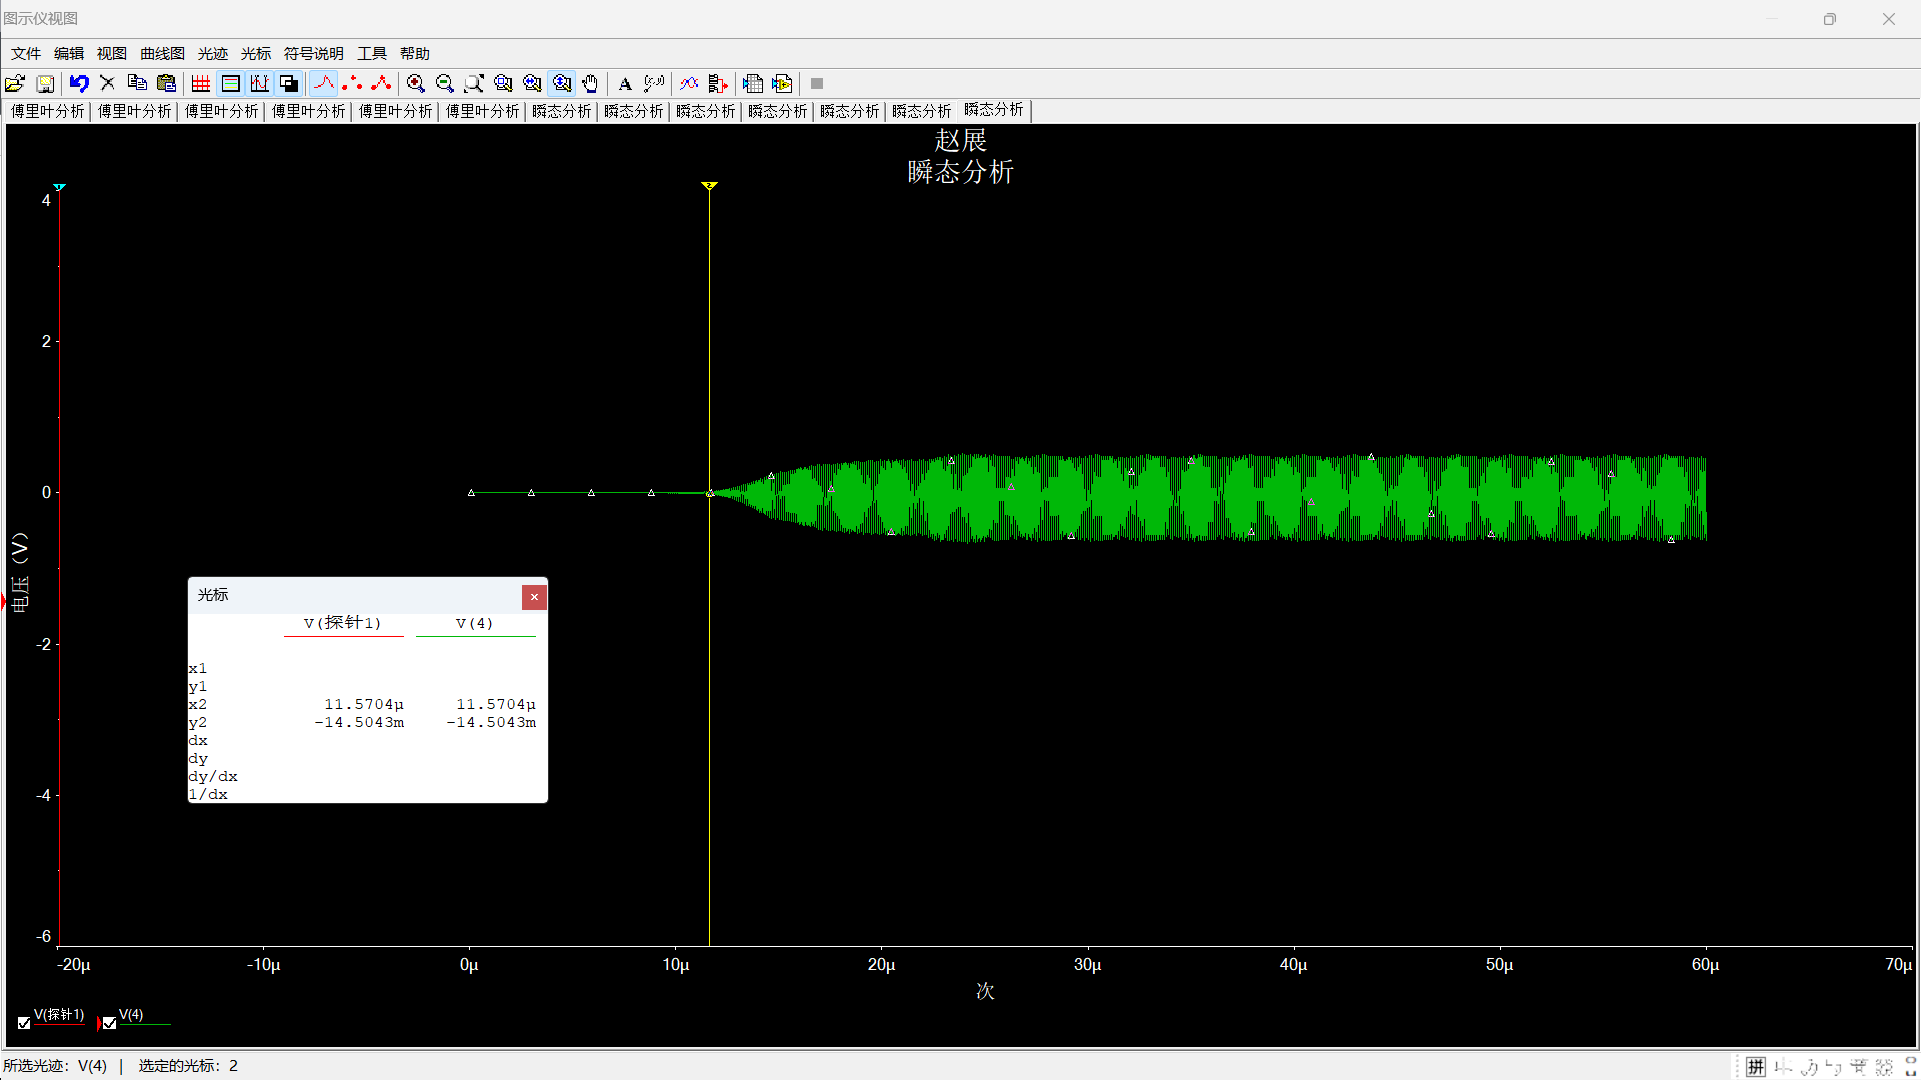
\includegraphics[width=0.6\textwidth]{6.png}
    \caption{瞬态分析:反馈系数$F=\frac{1}{2}$}
    \label{img:6}
\end{figure}
\begin{figure}[htbp]
    \centering
    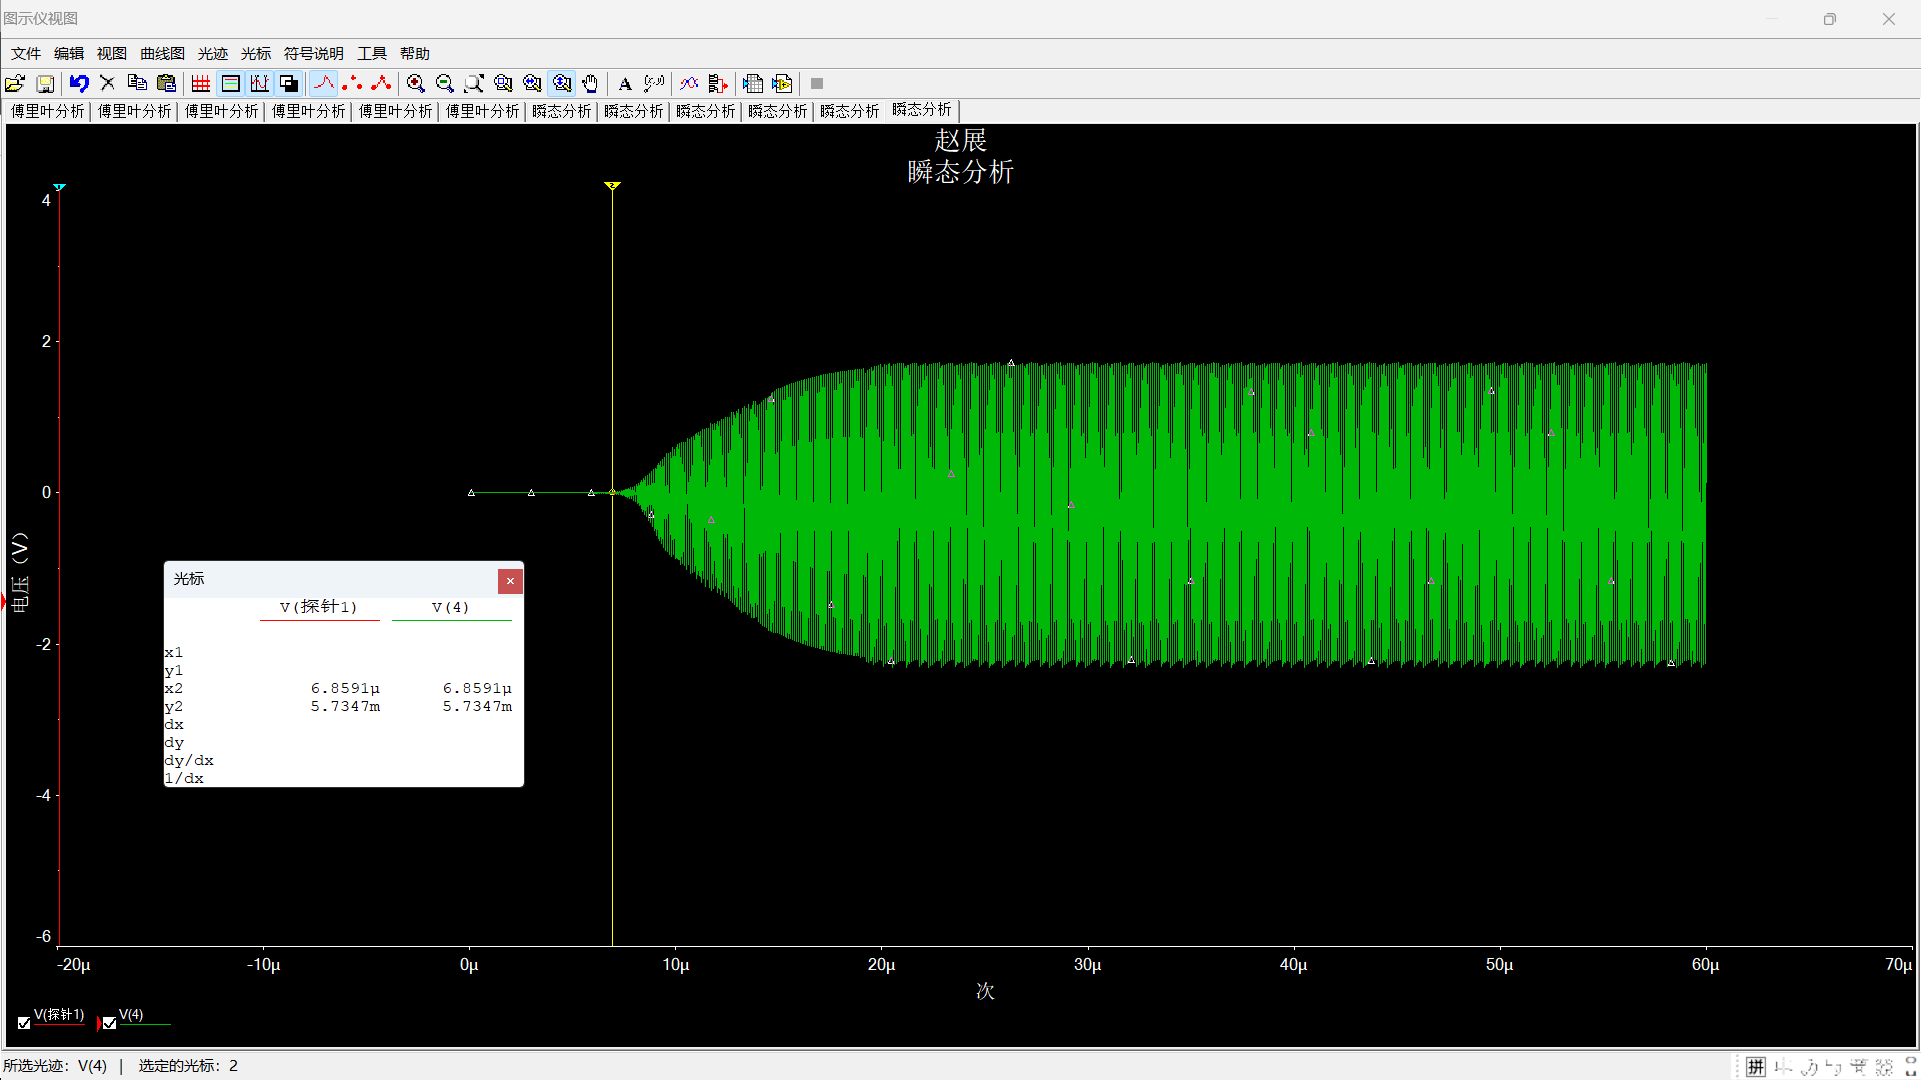
\includegraphics[width=0.6\textwidth]{7.png}
    \caption{瞬态分析:反馈系数$F=\frac{1}{4}$}
    \label{img:7}
\end{figure}
\begin{figure}[htbp]
    \centering
    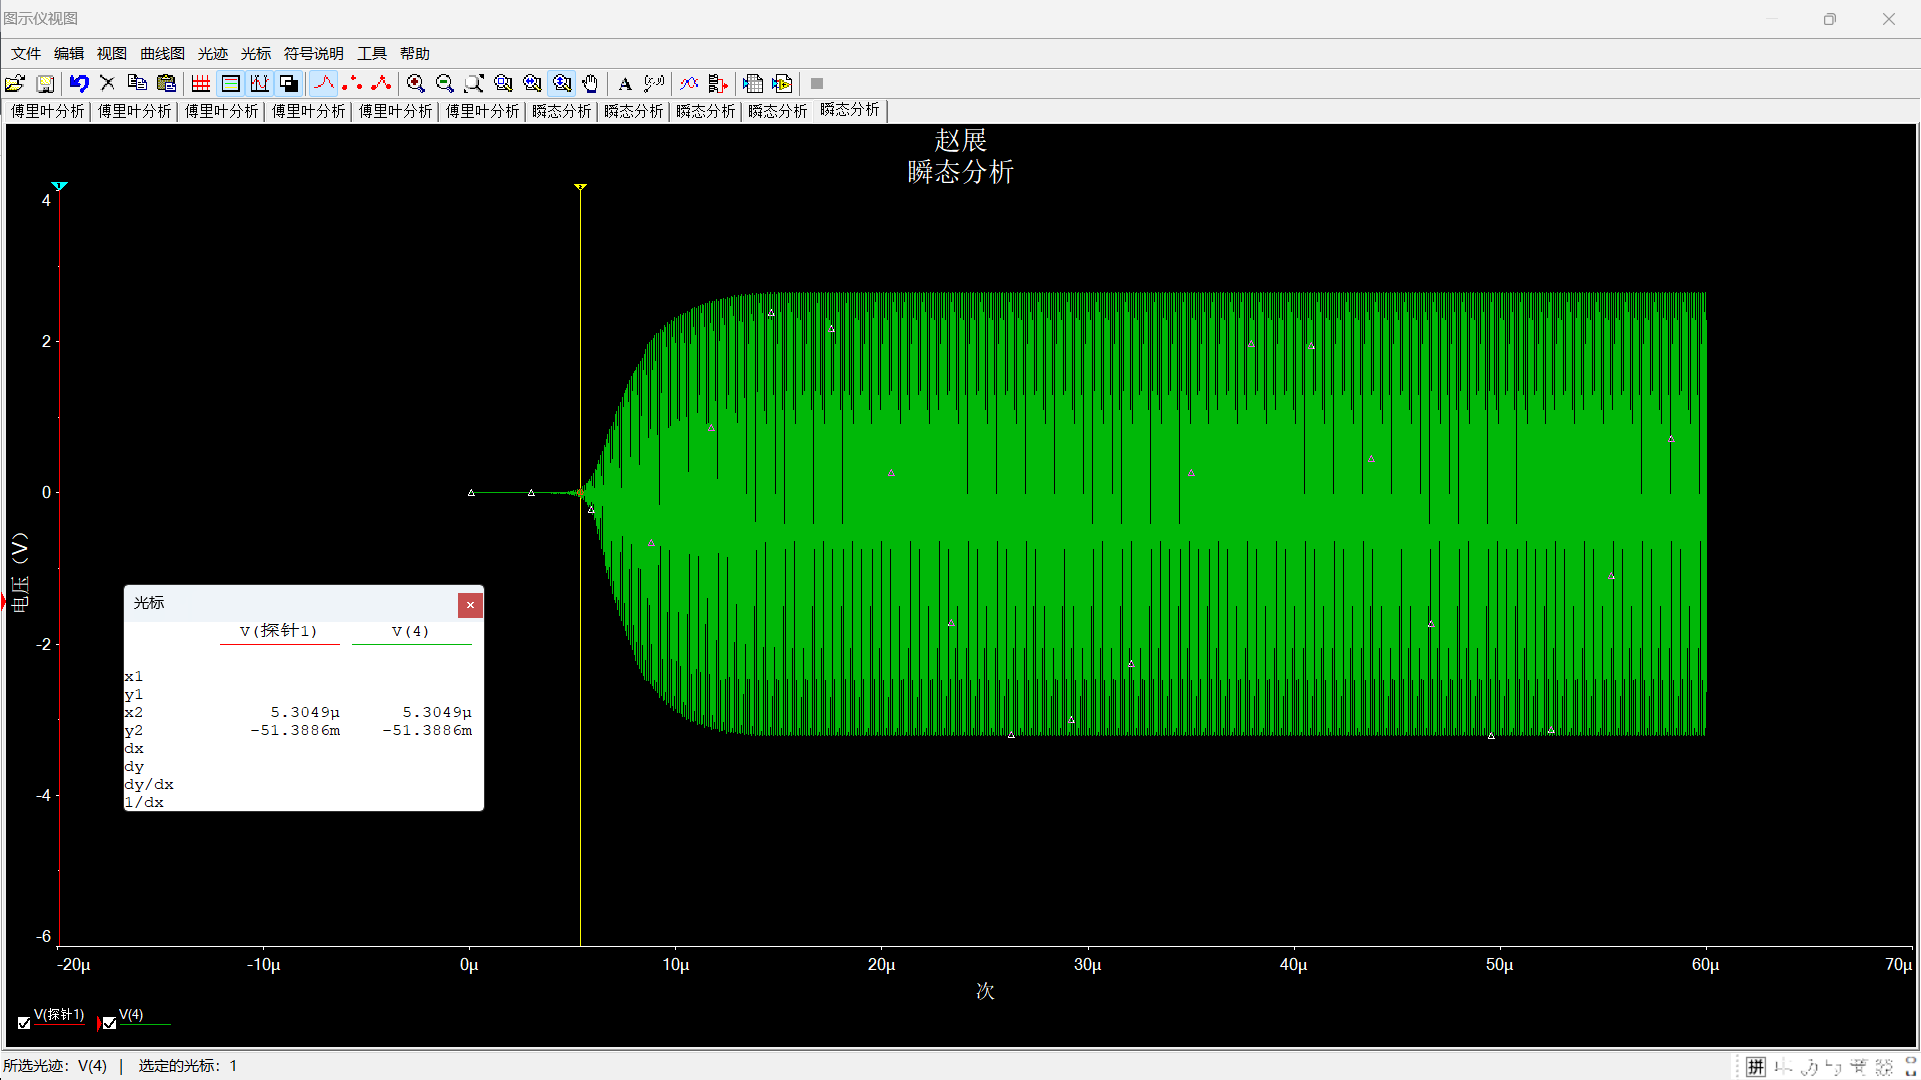
\includegraphics[width=0.6\textwidth]{8.png}
    \caption{瞬态分析:反馈系数$F=\frac{1}{8}$}
    \label{img:8}
\end{figure}
通过改变$C_1$的值来改变F,进行瞬态分析,查看起振时间和F的关系。
\paragraph{当$F=\frac{1}{2}$时}~{}\par
$C_1=F*C_2=250pF$,调整之后得到如图\ref{img:6}所示的结果
\paragraph{当$F=\frac{1}{4}$时}~{}\par
$C_1=F*C_2=125pF$,调整之后得到如图\ref{img:7}所示的结果
\paragraph{当$F=\frac{1}{8}$时}~{}\par
$C_1=F*C_2=62.5pF$,调整之后得到如图\ref{img:8}所示的结果
可以观察到,随着反馈系数F的降低,起振的时间不断变小
\subsubsection{$C_3$作用分析}

\begin{figure}[htbp]
    \centering
    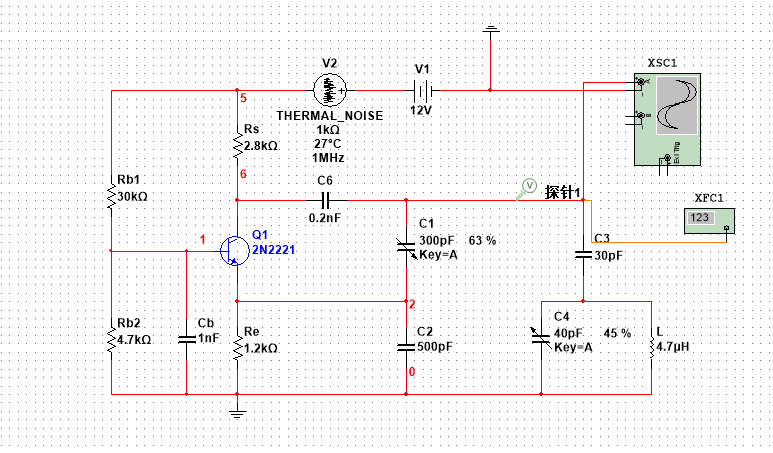
\includegraphics[width=0.6\textwidth]{9.png}
    \caption{电路中添加频率计数器}
    \label{img:9}
\end{figure}
\begin{figure}[htbp]
    \centering
    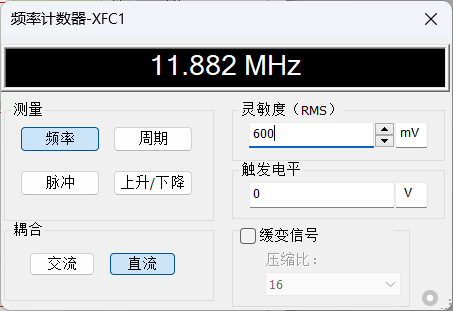
\includegraphics[width=0.6\textwidth]{10.png}
    \caption{频率计数器:$C_4$取25\%}
    \label{img:10}
\end{figure}
\begin{figure}[htbp]
    \centering
    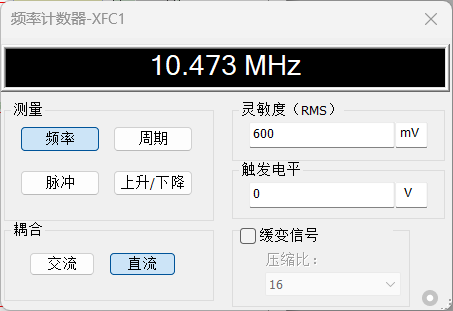
\includegraphics[width=0.6\textwidth]{11.png}
    \caption{频率计数器:$C_4$取50\%}
    \label{img:11}
\end{figure}
\begin{figure}[htbp]
    \centering
    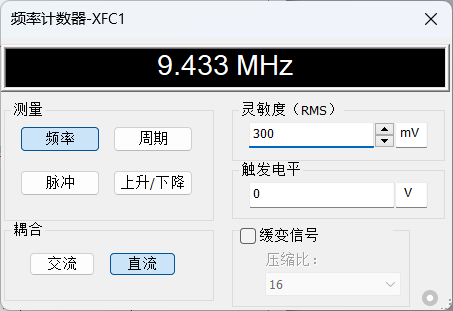
\includegraphics[width=0.6\textwidth]{12.png}
    \caption{频率计数器:$C_4$取75\%}
    \label{img:12}
\end{figure}
不断改变$C_4$的值,代替$C_3$值的变化,在电路中增加如图\ref{img:9}所示的频率计数器,仿真查看振荡频率。
\paragraph{$C_4$取25\%时}~{}\par
得到如图\ref{img:10}所示的仿真结果
\paragraph{$C_4$取50\%时}~{}\par
得到如图\ref{img:11}所示的仿真结果
\paragraph{$C_4$取75\%时}~{}\par
得到如图\ref{img:12}所示的仿真结果。

可以得出$C_3$的改变并不会影响反馈系数,但是会影响振荡频率。
\subsection{并联型晶体振荡器}
\subsubsection{输出信号波形与频谱分析}
使用并联晶体振荡器的仿真电路,使用瞬态分析得到输出信号的时域波形如图\ref{img:13}所示
\begin{figure}[htbp]
    \centering
    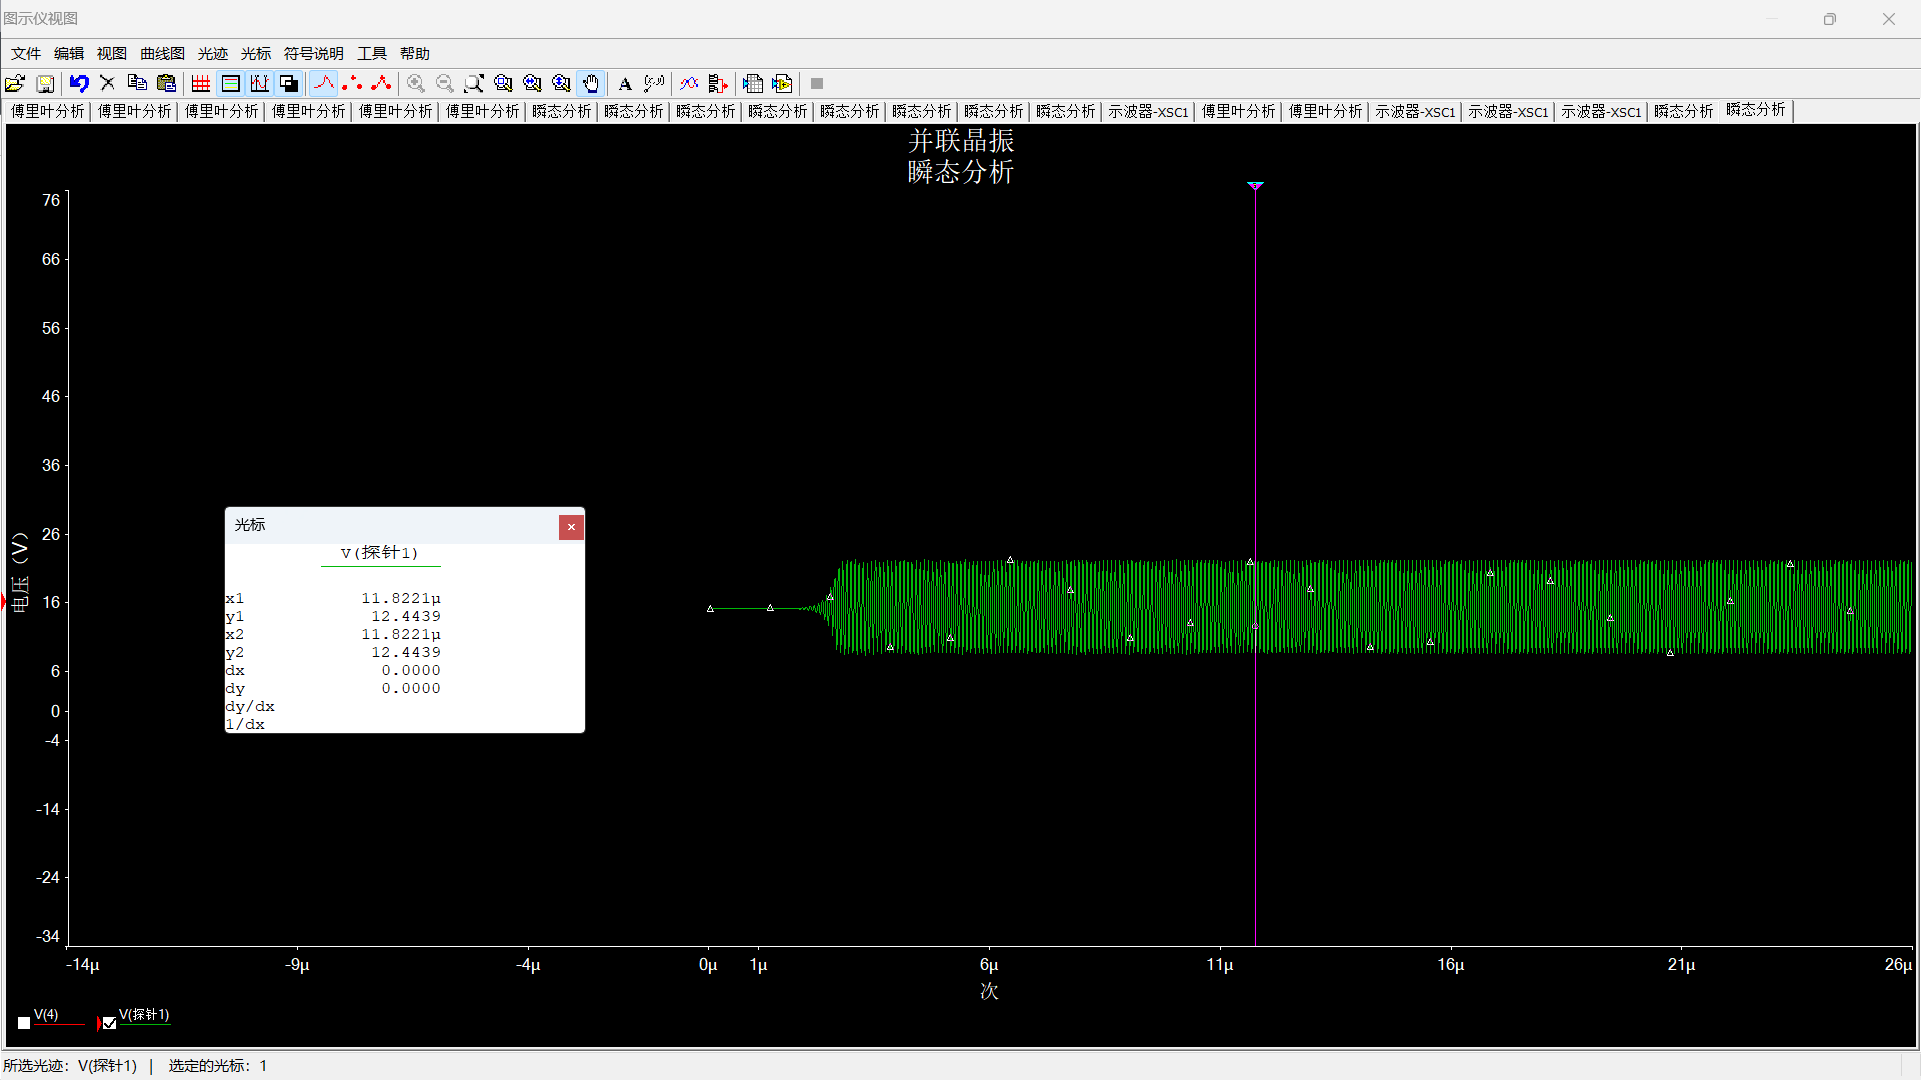
\includegraphics[width=0.8\textwidth]{13.png}
    \caption{瞬态分析:晶振电路输出电压信号波形}
    \label{img:13}
\end{figure}
对输出信号进行傅里叶分析,得到如图\ref{img:14}所示的结果
\begin{figure}[htbp]
    \centering
    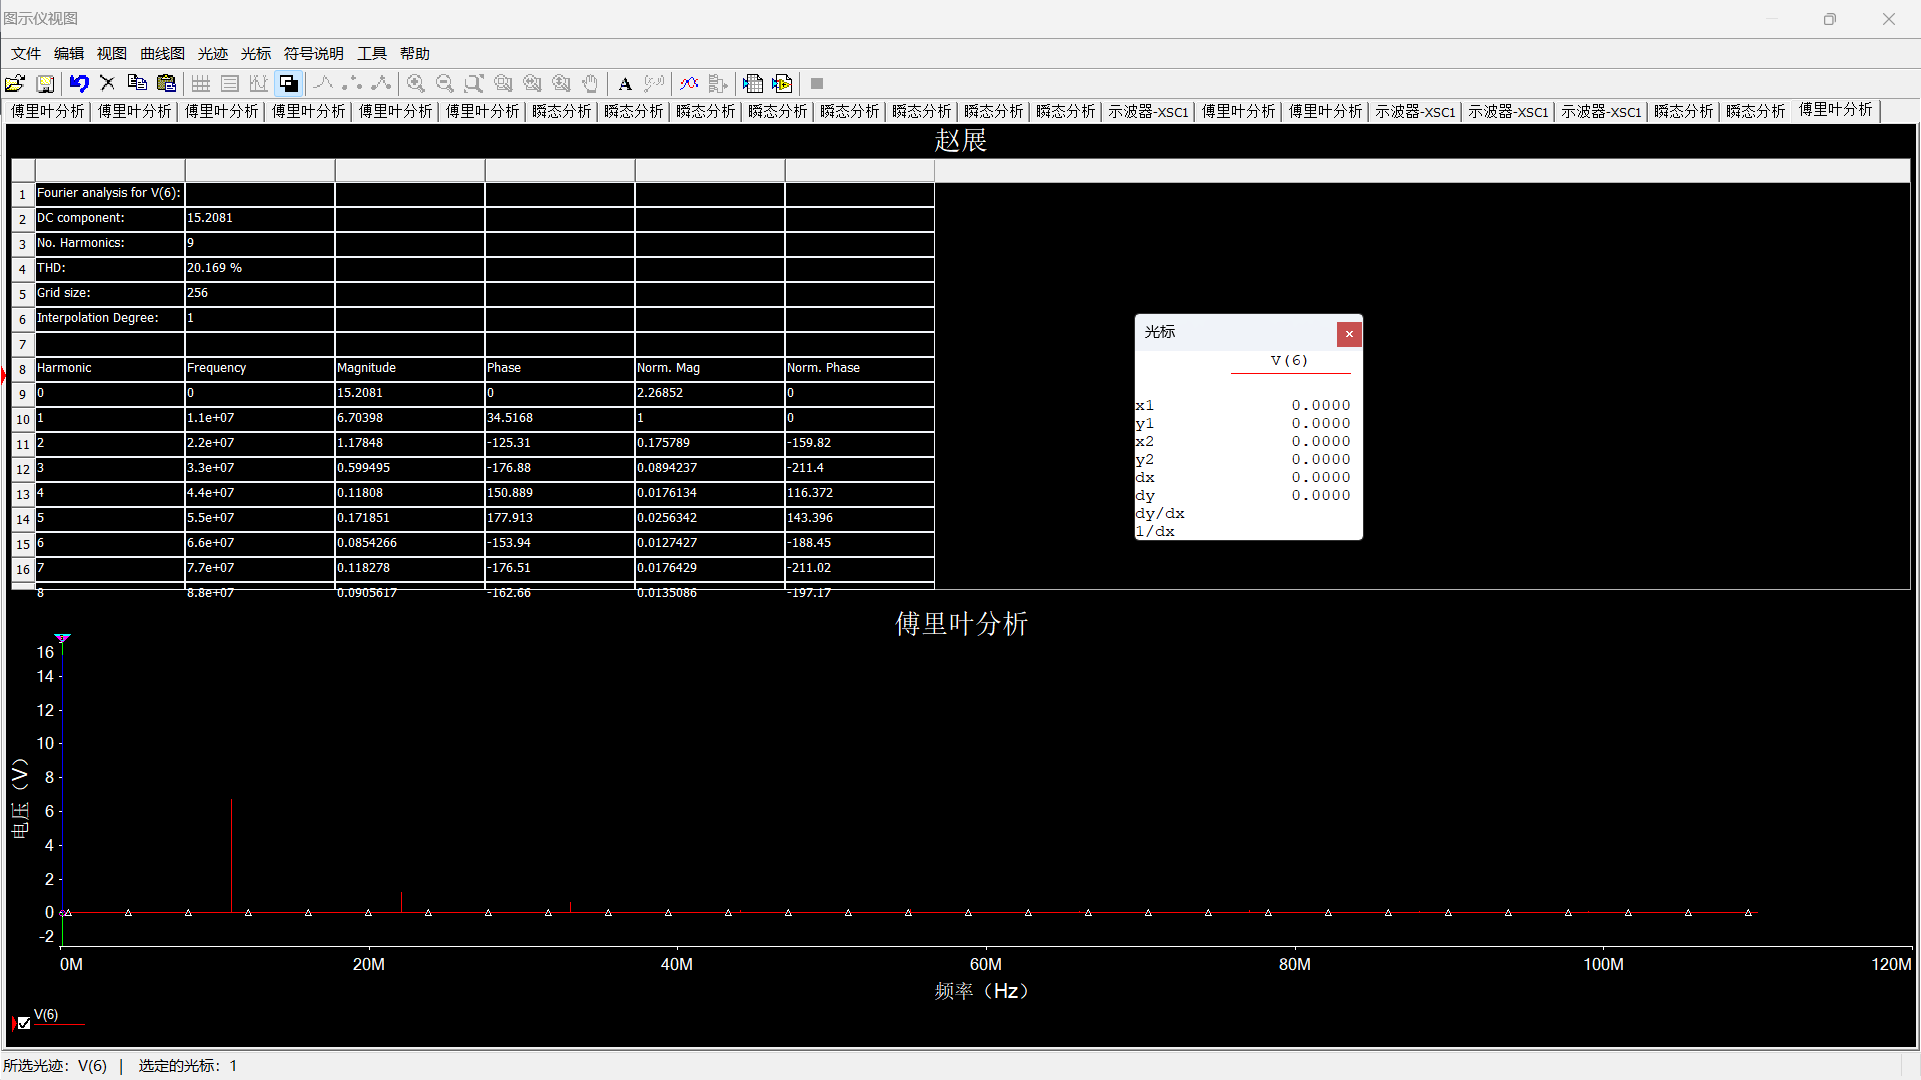
\includegraphics[width=0.8\textwidth]{14.png}
    \caption{傅里叶分析:晶振电路输出电压信号频谱}
    \label{img:14}
\end{figure}
可以看到输出信号的频谱大约在11.02MHz处。满足在10MHz以上。
\begin{figure}[htbp]
    \centering
    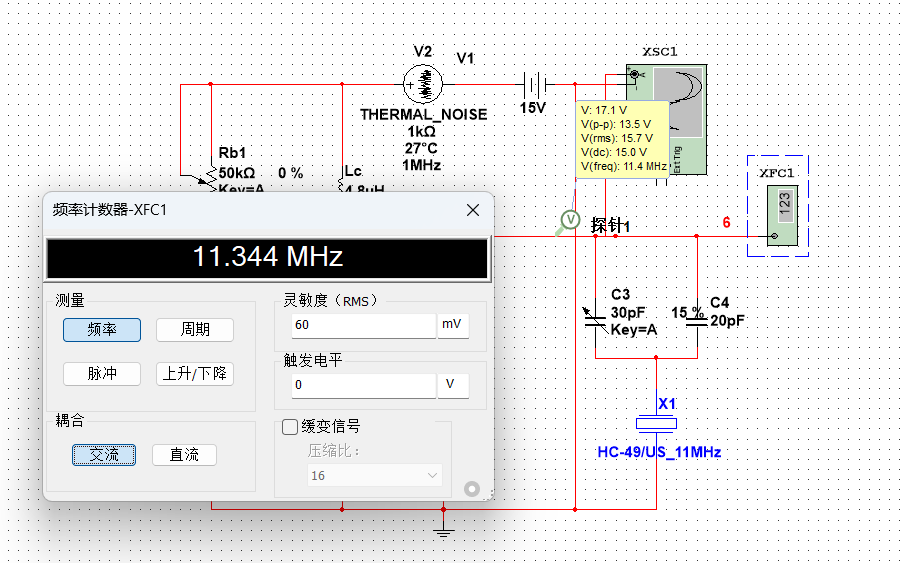
\includegraphics[width=0.8\textwidth]{15.png}
    \caption{频率计数器:晶振电路输出电压信号频率}
    \label{img:15}
\end{figure}
若使用频率计数器则如图\ref{img:15}所示
\newpage
\section{实验小结}
通过本次实验,我对Multisim的使用有了更深的了解,比如白噪声的引入等等,同时我也是重新更加深入学习了LC振荡器的使用,对这方面的知识进行了进一步的巩固。
通过这次实验,我也是将晶振电路和纯元器件电路进行对比,得到晶振电路性能更好这一结论。














\end{document}